\documentclass[A4paper,oneside,fleqn,11pt]{article}

% This first part of the file is called the PREAMBLE. It includes
% customizations and command definitions. The preamble is everything
% between \documentclass and \begin{document}.

%Cambiamos un poquito los márgenes%
\addtolength{\oddsidemargin}{-1in}
\addtolength{\evensidemargin}{-1in}
\addtolength{\textwidth}{2in}
\addtolength{\topmargin}{-1in}
\addtolength{\textheight}{2in}



\usepackage{mathtools}
\usepackage{graphicx}              % to include figures
\usepackage{amsmath}               % great math stuff
\usepackage{amsmath,scalerel}
\usepackage{amsfonts}              % for blackboard bold, etc
\usepackage{amsthm}                % better theorem environments
\usepackage{amssymb}
\usepackage{mathrsfs}
\usepackage[spanish]{babel}
\usepackage[utf8]{inputenc}
\usepackage{hyperref}
\usepackage{multicol}
\usepackage{tikz-cd}
\usepackage{amsmath}
\usepackage[linesnumbered,ruled]{algorithm2e}
\usepackage{algpseudocode}
\usetikzlibrary{calc}
\usetikzlibrary{matrix}
\usepackage{graphicx,wrapfig,lipsum}
\usepackage{subcaption} %para poner varias imagenes en un figure
\usepackage{graphicx} % Required for including pictures

\usepackage{sidecap}%para poner la descripción de una imagen al lado de la imagen,no abajo ni arriba
\usepackage{float} % Allows putting an [H] in \begin{figure} to specify the exact location of the figure
\usepackage{wrapfig} % Allows in-line images such as the example fish picture
\graphicspath{ {Grphs/} }


\setcounter{tocdepth}{3}% to get subsubsections in toc

\let\oldtocsection=\tocsection

\let\oldtocsubsection=\tocsubsection

\let\oldtocsubsubsection=\tocsubsubsection

% various theorems, numbered by section

\newtheorem{teo}{Teorema}[section]
\newtheorem{lem}[teo]{Lema}
\newtheorem{prop}[teo]{Proposición}
\newtheorem{cor}[teo]{Corolario}
\newtheorem{crit}[teo]{Criterio}
\newtheorem{propi}[teo]{Propiedad}

\theoremstyle{definition}
\newtheorem{ejcio}[teo]{Ejercicio}
\newtheorem{conj}[teo]{Conjetura}
\newtheorem{obs}[teo]{Observación}
\newtheorem{defn}[teo]{Definición}
\newtheorem{ax}[teo]{Axioma}
\newtheorem{ex}[teo]{Ejemplo}

\newcommand{\bd}[1]{\mathbf{#1}}  % for bolding symbols
\newcommand{\cl}[1]{\overline{#1}} 
\newcommand{\CC}{\mathbb{C}}
\newcommand{\RR}{\mathbb{R}}      % for Real numbers
\newcommand{\ZZ}{\mathbb{Z}}      % for Integers
\newcommand{\NN}{\mathbb{N}}
\newcommand{\QQ}{\mathbb{Q}}
\newcommand{\FF}{\mathbb{F}}
\newcommand{\col}[1]{\left[\begin{matrix} #1 \end{matrix} \right]}
\newcommand{\comb}[2]{\binom{#1^2 + #2^2}{#1+#2}}
\newcommand{\eps}{\varepsilon}
\renewcommand{\hom}{\mathrm{Hom}}
\let\oldemptyset\emptyset
\let\emptyset\varnothing
\DeclareMathOperator{\id}{id}
\DeclareMathOperator{\mcm}{mcm}
\DeclareMathOperator{\mcd}{mcd}
\DeclareMathOperator{\ord}{ord}
\DeclareMathOperator{\im}{im}
\DeclareMathOperator{\End}{End}
\DeclareMathOperator{\Aut}{Aut}
\DeclareMathOperator{\sg}{sg}
\DeclareMathOperator{\cok}{cok}
\DeclareMathOperator{\ext}{Ext}
\DeclareMathOperator{\Obj}{Obj}
\DeclareMathOperator{\rank}{rk}
\DeclareMathOperator{\gr}{gr}
\DeclareMathOperator{\car}{char}
\DeclareMathOperator{\Nil}{Nil}
\DeclareMathOperator{\spec}{Spec}
\DeclareMathOperator{\ev}{ev}
\DeclareMathOperator{\ann}{Ann}
\DeclareMathOperator{\tr}{Tr}
\DeclareMathOperator*{\bigcdot}{\scalerel*{\cdot}{\bigodot}}
\def\acts{\curvearrowright}
\def\stca{\curvearrowleft}

\setcounter{tocdepth}{10}
\setcounter{secnumdepth}{10}

\usepackage[utf8]{inputenc}
\usepackage{fancyhdr}


\begin{document}

%----------------------------------------------------------------------------------------
%	TITLE PAGE
%----------------------------------------------------------------------------------------

\begin{titlepage}

\center % Center everything on the page

\newcommand{\HRule}{\rule{\linewidth}{0.5mm}} % Defines a new command for the horizontal lines, change thickness here

\textsc{\LARGE Universidad de Buenos Aires}\\[1.5cm] % Name of your university/college
\textsc{\Large Facultad de Ciencias Exactas y Naturales}\\[0.5cm] % Major heading such as course name
\textsc{\large Departamento de Computación}\\[0.5cm] % Minor heading such as course title
\textsc{\large Algoritmos y Estructuras de Datos III}\\[0.5cm] % Minor heading such as course title

\HRule \\[0.8cm]
{ \huge \bfseries Trabajo Práctico 3}\\[0.4cm] % Title of your document
\HRule \\[1.5cm]

\begin{minipage}{0.8\textwidth}
\center
%\begin{flushleft} 
\Large
\emph{Autores:}


{Nicolás Chehebar, mail: \textit{nicocheh@hotmail.com}, LU: 308/16 

Matías Duran, mail: \textit{mato\_ fede@live.com.ar}, LU: 400/16 

Lucas Somacal, mail: \textit{lsomacal@gmail.com}, LU: 249/16} % Your name
%\end{flushleft}
~
\end{minipage}\\[4cm]

%\includegraphics{Logo}\\[1cm] % Include a department/university logo - this will require the graphicx package

\vfill % Fill the rest of the page with whitespace

\end{titlepage}

%----------------------------------------------------------------------------------------
%	TABLE OF CONTENTS
%----------------------------------------------------------------------------------------


 %\chead{Algo III, TP2, Chehebar, Duran, Somacal}
 
%\title{Algoritmos y Estructuras de Datos III, TP2}
%\author{Nicolás Chehebar, Matías Duran, Lucas Somacal}
%\date{}



\pagenumbering{roman}
\pagenumbering{arabic}
%\maketitle
\tableofcontents
\clearpage







\section{El Juego}
\subsection{Descripción}
El juego es una generalización del popular 4 en línea \footnote{$https://es.wikipedia.org/wiki/Conecta_4$}. Consiste en una grilla de $M$ filas y $N$ columnas en la cual dos jugadores colocan alternadamente una ficha propia (identificada con rojo las de un jugador y azul las del otro). Las fichas se pueden colocar en cualquier columna de la grilla y una vez elegida la columna, esta determina el movimiento, ya que irá a la fila de "más abajo" (la de numeración más baja) que esté desocupada. El objetivo de un jugador será lograr tener un línea recta (diagonal, vertical u horizontal) de $C$ fichas propias. Cuando esto suceda, el jugador ganará el partido. Además, cada jugador dispone de $P$ fichas. En caso de que ambos se queden sin fichas y ninguno haya ganado, la partida finaliza en empate. También se da un empate si la grilla queda llena (y ninguno había ganado). Se trata de una generalización del 4 en línea ya que si tomamos parametros $M=6, N=7, C=4, P=21$ se replicarían las condiciones iniciales del juego.
\subsubsection{Ejemplos}































\section{Jugador Óptimo}

\subsection{El algoritmo}

El algoritmo del jugador del punto 1.a brinda un jugador óptimo. Nos asegura que este jugador hará la estrategia ganadora si hubiera. En caso de que esta no exista, realizará una de empate. Y si tampoco existiera esa, jugará indistintamente sabiendo que perderá. Este análisis se realiza jugada a jugada. Para ejemplificar esto, podría suceder que el oponente tenga la estrategia ganadora y en ese caso nuestro jugador hará cualquier movida indistintamente (pues sabe que perderá), pero si en la próxima jugada el oponente no realiza la correspondiente a su estrategia ganadora y da un nuevo estado del tablero en el que esta vez nuestro jugador tiene estrategia ganadora, nuestro jugador jugará y ganará ya que ahora sí tiene estrategia ganadora.

Para lograr esto, utilizamos una técnica algorítmica similar al Backtracking en el sentido de que exploramos todas las soluciones posibles y nos quedamos con la óptima. Pero esta vez tenemos dos jugadores interviniendo en la situación donde lo que uno busca es todo lo contrario a lo que busca el otro. Podemos decir que un tablero finalizado tiene 3 puntajes posibles, 1 si ganamos nosotros, 0 si es empate, -1 si ganó el otro (podríamos sino generalizarlo para todo tablero y que haya un cuarto valor que sea inválido si aún no hemos calculado el valor de dicho tablero). Así, lo que sabemos es que turno a turno, uno quiere maximizar el puntaje y el otro minimizarlo. Es por esto que dicha técnica algorítmica se llama Minimax. 

De esta manera, igual que en Backtracking tenemos un arbol de ejecución donde cada nodo es un estado del tablero y la raiz es el tablero vacío. Cada nodo (que no sea hoja) tendrá $N$ hijos donde cada uno representará que la próxima jugada fue en alguna de las $N$ columnas. De esta forma, recorremos todos los tableros posibles. Según quién comience, en el primer nivel trataremos de maximizar o minimizar, en el siguiente lo contrario y así sucesivamente. Todos los niveles impares minimizarán si empieza el contrincante y maximizarán si empieza nuestro jugador. El que maximiza le asignará a su nodo un puntaje que será el máximo de los puntajes de todos sus hijos. Análogamente el que minimiza le asignará a su nodo un puntaje que será el mínimo de los puntajes de todos sus hijos.

Así, ejecutando dicho algoritmo la raíz tendrá la información de quién tiene la estrategia ganadora, o que ambos pueden asegurar el empate según quién empiece y haya un 1, 0 o -1. Esta es la idea general del algoritmo, lo veremos más claro en el siguiente pseudocódigo

\subsubsection{El Pseudocódigo}


\subsection{La poda alfa-beta}


\subsubsection{El algoritmo}

\subsubsection{El Pseudocódigo}



\subsection{Complejidad}





\subsection{Experimentación}

\subsubsection{Contexto} 


La experimentacion se realizó toda en la misma computadora, cuyo procesador era Intel Atom$\texttrademark$ CPU N2600 @ 1.60GHz, de 36 bits physical, 48 bits virtual, con una memoria RAM de 2048 MB.  Para experimentar, se calculó el tiempo que tardaba el algoritmo sin considerar el tiempo de lectura y escritura ni el tiempo que llevaba armar la matriz (ya que se leía un dato, se escribía la matriz y luego se leía el siguiente). 
El tiempo se medía no como tiempo global sino como tiempo de proceso, calculando la cantidad de ticks del reloj (con el tipo clock\_t de C++) y luego se dividía el delta de ticks sobre CLOCKS\_PER\_SEC. En todos los experimentos el tiempo se mide en segundos. 

\subsubsection{Sin poda}
En principio, para verificar experimentalmente que el jugador era óptimo se jugo en tableros pequeños (particularmente de $2\times2, 3\times3, 2\times3, 3\times2, 2\times4, 4\times2, 3\times4, 4\times3$) con un $c=2, 3, 4$ siempre que cumpla la condicion del juego ($c\leq min{N,M}$) contra el jugador random. En todos los casos la cantidad de iteraciones fue de $2*3\textsuperscript{(N*M)}$ por lo que todo tablero posible tenía una probabilidad considerable de ser jugado (notar que la cantidad de juegos posibles es menor que  $N\textsuperscript{(N*M)}$ -de hecho es menor que $3\textsuperscript{(N*M)}$ ya que cada casilla tiene o bien nada o ficha de un jugador o del otro-). Tomamos esta cantidad de repeticiones ya que a cada paso lo que se elije es una de $N$ -o menos si hay columnas llenas- opciones donde jugar y esto se repite hasta que termine el juego -a lo sumo se lena la grilla $N*M$ veces-. Así, tenemos tantas iteraciones como secuencias posibles de jugadas, o sea partidas en general. Como el jugador es random equiprobable, la distribución respecto de que jugada de las posibles realizar es uniforme y lo multiplicamos por dos para que sea más probable que salga cualquier partida posible (estamos jugando toda partida posible con una probabilidad considerable). Más aún, es una probabilidad bastante alta ya que se puede notar que solo queremos contar todas las opciones de secuencias de jugadas que puede dar el segundo jugador (en este caso el aleatorio), lo que nos provee una cota menor de la cantidad total de jugadas distintas que se le pueden hacer al jugador optimo, acotandolo por $N\textsuperscript{(N*M/2)}$. 

Estos experimentos se repitieron en dos casos cada uno, cuando comenzaba el minimax y cuando comenzaba el random. Además para fijado el jugador que empieza, se repitió con valores de fichas que fueron $p=N*M/2, N*M/3, N*M/4$ donde el primer valor de p aseguraba que se pueda jugar sin limite de fichas (siempre se podría llegar a llenar el tablero) y los otros dos sí imponian un limite de fichas. Luego de cada experimento, nos fijamos en el archivo .log devuelto por dichas iteraciones y en todos se observo el mismo comportamiento:
\begin{itemize}
\item O bien siempre ganaba (lo que nos indica que había estrategia ganadora para el que empieza). Al invertir la situación (cambiar el jugador que empieza), se daba el item 3.
\item O bien siempre ganaba o empataba (lo que nos indicaria que la mejor estrategia para ambos resulta en un empate, pero como el jugador random no siempre juega lo mejor, le daba la posibilidad a nuestro jugador de ganar). Al invertir la situación (cambiar el jugador que empieza) se obtenía este mismo item.
\item O bien siempre ganaba o empataba o perdía (lo que nos indicaría que el que no empieza tiene estrategia ganadora, pero como el jugador random no siempre juega lo mejor, le daba la posibilidad a veces a nuestro jugador de ganar). Al invertir la situación (cambiar el jugador que empieza), se daba el item 1.
\end{itemize}

Como se explico, estas situaciones, en todos estos tableros reforzaron fuertemente la idea de que se trataba de un jugador óptimo. Cabe aclarar que se realizo solo con tableros pequeños debido a que para tableros muy grandes el jugador demoraba demasiado tiempo en decidir que jugar (como se vio en la complejidad teórica exponencial, por lo que crecía brutalmente al crecer el tamaño del tablero y la cantidad de columnas) y por ende resultaba inviable realizar una alta cantidad de iteraciones para recorrer una gran cantidad de tableros posibles lo que nos permita reforzar la idea de optimalidad del jugador. 

Pero en tableros pequeños hemos podido comprobar que en todos los tableros que se dieron, cumplieron que el jugador era óptimo ya que si tenía la posibilidad de ganar lo hacía, en caso de no existir esta, si tenía la posibilidad de empatar lo hacía y recién en caso de no existir esta, jugaba cualquier cosa sabiendo perdería.  Pero como hemos visto, esto se comprobaba paso a paso, por lo que el jugador podía jugar creyendo que perdería y como el otro no jugo optimamente luego, pasar a poder ganar o empatar (y efectivamente hacerlo pues es optimo); o sea, asume optimalidad del rival.

Esta experimentación nos permitió reforzar nuestra idea (al menos para estos tableros pequeños y con una probabilidad muy alta) de que el jugador era efectivamente óptimo.

Para tratar de reforzar experimentalmente la complejidad teorica deducida previamente, se realizo una experimentación en la que se registró para varios tableros de tamaño pequeño (de $2\times2, 3\times3, 4\times4, 2\times3, 3\times2, 2\times4, 4\times2, 5\times2, 2\times5, 2\times6, 2\times7, 2\times8, 6\times2, 7\times2, 8\times2, 3\times4, 4\times3, 3\times5, 5\times3$) ya que para tamaños mayores los tiempos de ejecución fueron inabordables (lo que reforzó en parte la complejidad teorica esperada). Para cada uno de esos tableros, se jugo con fichas de sobra (mas que la cantidad que entraba en el tablero, 88 particularmente) y el $c$ se movio entre $2, 3$ y $4$ siempre y cuando se cumplieran las condiciones del juego. Siempre se jugo contra el jugador random provisto por la cátedra (que con distribucion uniforme decidía aleatoriamente en cual de las $N$ posibles columnas jugar). Para asegurar distintas configuraciones, se repitió cada partido $10$ veces. 


Para todos estos juegos se registró a cada jugada del algoritmo el tiempo de ejecución que este tomó en decidir que jugada realizar y se registró una variable que reflejaba un refinamiento de la complejidad esperada. Esta variable se definió como $a^b$ donde $a=|Columnas Donde Es Posible Jugar|$ y $b =|Casillas Libres En El Tablero|$ que es en particular acotable por $N\textsuperscript{(N*M)}$. Luego, se graficó el $tiempo/(a^b)$ en funcion de $a^b$ y se esperaría obtener un grafico acotable por una constante lo que reforzaría la idea de que el aloritmo cumpía la cota propuesta. Se graficó esto en la Figura 1, (junto con su análogo con el algoritmo con poda) y efectivamente se cumplió con lo esperado ya que se ve que el gráfico es prácticamente constante salvo en los primeros valores, lo que tiene sentido y refuerza aún más la hipotesis, porque para esos valores toman mucha más importancia los términos constantes que no dependen de la variable propuesta como complejidad. Al aumentar la variable propuesta, la importancia del termino constante se reduce y pasa a ser constante. Más aún, esa constante es $0$, lo que nos indica que es incluso menor a la complejidad propuesta (o sea que cumple lo pedido, ya que en particular es menor, que es a lo que apunta la notacion $\mathcal{O}$) ya que este método de dividir por la complejidad esperada es muy sensible, ya que da una constante si dividimos por algo que cumpla ser $\theta$, y sino ante una pequeña alteración en la complejidad se refleja claramente en el gráfico (o bien pasa a ser creciente o decreciente). Tiene sentido que sea menor ya que muchas veces el partido termina antes de que completemos efectivamente el tablero (que es la cota que propusimos) y además no siempre tenemos tantas opciones como columnas posibles de jugar ahora (cota que propusimos), sino que con el desarrollo del juego las opciones de columnas posibles van disminuyendo. Igualmente, esto nos permite reforzar claramente nuestra hipotesis de que cumple la complejidad teorica propuesta.

\subsubsection{Con poda}
En el caso con poda se realizo la misma experimentación para comprobar la optimalidad. Como el algoritmo tardaba un poco menos (por la poda realizada), se realizó (además de con los ya mencionados) con tableros de tamaño $4\times4, 3\times5, 5\times3, 4\times5, 5\times4, 3\times6, 3\times7$ , con los mismos valores de c que antes (y siempre y cuando cumpliera las condiciones del juego). También se varió la cantidad de fichas de la misma forma.

Nuevamente, los resultados y conclusiones sobre estos fueron las mismas, lo que nos permitió reforzar nuestra idea (al menos para estos tableros pequeños y con una probabilidad muy alta) de que el jugador era efectivamente óptimo.



\begin{wrapfigure}[10]{R}{0.4\textwidth}
	%\centering
	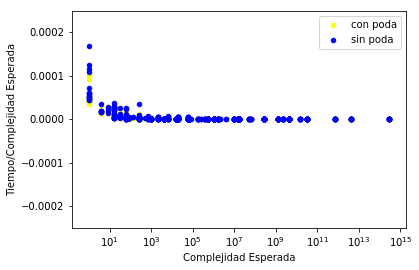
\includegraphics[width=0.4\textwidth]{complejidad1.png}
	\caption{ Gráfico de segundos de ejecución (de cada jugada) dividido $a^b$ en función de $a^b$ para los partidos jugados por el algoritmo con y sin poda en tableros pequeños contra el jugador random.}
\end{wrapfigure}


Para verificar que la poda efectivamente se ejecutaba y permitía podar varios niveles del arbol de ejecución del minimax, decidimos analizar el tiempo de ejecución ya que si no se analizaran estas partes podadas, el tiempo de ejecución sería menor. Por eso se ejecutó para las exactas mismas partidas con las que se experimento en sin poda, la misma cantidad de veces cada una, contra el mismo jugador (que era el jugador random) que es importante aclarar que como no era deterministico medimos en la misma partida (o sea, ambos algoritmos -con y sin poda- recibían el mismo tablero a cada jugada) el tiempo de ejecución de ambos (y finalmente jugaba el con poda la jugada -lo que nos resultaba poco relevante ya que queríamos medir tiempos de ejecución para distintos tableros y verificar nuestra complejidad que no dependía de como jugaban y tampoco era el objetivo analizar como jugaban-). Luego se compararon los dos tiempos medidos para las 688 jugadas en todos los partidos. Así, solamente fueron 9 jugadas en las que el algoritmo con poda tardo más que el sin poda y estas diferencias fueron realmente despreciables (tanto en cantidad de jugadas diferentes, como en diferencia de tiempo). Listamos a continuación los valores en los que difirieron (5.8e-05 contra 5.6e-05, 0.000383 contra 0.000352, 0.000212 contra 0.000202, 0.000535 contra 0.000251, 0.000282 contra 0.00027, 0.00028 contra 0.000264, 0.000469 contra 0.000459, 0.000417 contra 0.000355, 0.000341 contra 0.000323 -del algoritmo con poda contra el sin poda respectivamente-).


Esta experimentación nos permitió no solo reforzar nuestra hipótesis (justificada teoricamente en el algoritmo) de que el tiempo de ejecución era efectivamente menor, por lo que se ejecutaba la poda, sino también comprobar que se seguía manteniendo la complejidad teórica propuesta para el algoritmo con poda (ya que era la misma que la del algoritmo sin poda y hemos visto que el tiempo de ejecución era menor). Más aún esto se puede ver en la Figura 1 donde se ve que el algoritmo con poda nunca supera al algoritmo sin poda en tiempo de ejecución.



















\section{Jugador parametrizable}


\subsection{El algoritmo}

\subsubsection{El Pseudocódigo}



\subsection{Complejidad}



\subsection{Experimentación}

Si bien el grueso del análisis y experimentación sobre este jugador consistirá en buscar buenos parámetros que mejoren al jugador, consideramos relevante reforzar experimentalmente nuestra hipótesis de complejidad teórica esperada. Para esto tomamos mediciones análogas a las del jugador óptimo solo que jugando en más tableros. Se jugó en tableros que comprendían todas las combinaciones factibles con las columnas y filas moviendose entre $2$ y $10$, c moviendose entre $2$ y $\min{columnas,filas}$ y p moviendos entre $2$ y $filas*columnas/2$. En cada jugada, los parametros que determinaban la proxima jugada a realizar se sorteaban aleatoriamente. Todo esto fue para ver experimentalmente que la dependencia que proponíamos en la complejidad dependía efectivamente solo de n y m. Así, igual que antes, realizamos un grafico de tiempo de ejecucion/(filas*$columnas^2$) en funcion de filas*$columnas^2$ donde esperabamos obtener un gráfico constante que reforzaría nuestra hipótesis de que la complejidad (como se justifico teóricamente) era de $\mathcal{O}(N^2 M)$. Este gráfico se puede ver en la Figura 2



\begin{wrapfigure}[10]{L}{0.4\textwidth}
	%\centering
	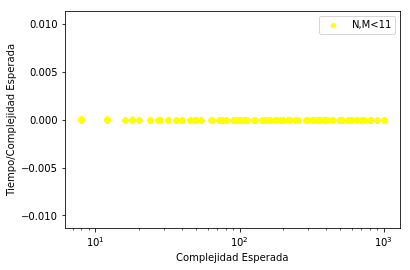
\includegraphics[width=0.4\textwidth]{complejidad2.png}
	\caption{ Gráfico de segundos de ejecución (de cada jugada) dividido $N^2 *M$ en función de $N^2 * M$ para los partidos jugados por el jugador que utiliza la funcion parametrizable a cada paso. Varian c y p. Columnas y filas menores a 11.}
\end{wrapfigure}

Efectivamente como se puede ver en la Figura 2, pareciera cumplirse la complejidad esperada ya que el gráfico es practicamente constante. Más aún,  al variar por todas sus posibilidades c, p y el parametro de la función, esto refuerza la hipotesis (que se justifico en la explicación del algoritmo) de que esta cota de dependencia no se ve afectada por el parámetro en particular, o la cantidad de fichas que queden, o el c. Sabiendo esto, tenemos la posibilidad de experimentar para tableros de mayor tamaño (ya que no tenemos que repetirlos para distintos c y p). Por esto, se experimento con un c aleatorio (con distribución uniforme, usando rand() de C++) entre 2 y min(columns,rows)  y p=N*M/2 para que no se interrumpa el partido por falta de fichas  y se vario nuevamente las filas y columnas pero ahora el limite superior paso a ser 20 en vez de 10. Nuevamente, se realizo el mismo gráfico que antes con los nuevos datos que se puede ver en la Figura 3.

\begin{wrapfigure}[10]{R}{0.4\textwidth}
	%\centering
	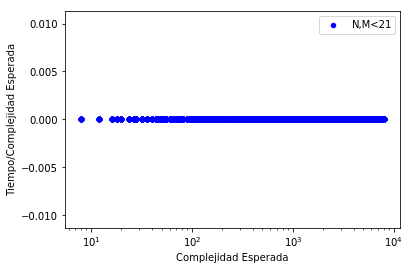
\includegraphics[width=0.4\textwidth]{complejidad2b.png}
	\caption{ Gráfico de segundos de ejecución (de cada jugada) dividido $N^2 *M$ en función de $N^2 * M$ para los partidos jugados por el jugador que utiliza la funcion parametrizable a cada paso. Columnas y filas menores a 51.}
\end{wrapfigure}

Podemos ver en el gráfico de la Figura 3, que los resultados siguen siendo los mismos incluso para tableros de tamaño mayor.  Nuevamente el gráfico es prácticamente una constante. El análisis y su justificación es totalmente análogo al realizado en la Figura anterior (la 2) y al ser con tamaños de entrada mayores, refuerza más aún experimentalmente la complejidad que fue propuesta teóricamente.






\section{Grid Search}



\subsection{El algoritmo}

\subsubsection{El Pseudocódigo}



\subsection{Experimentacion}


















\section{Algoritmo Genético}



\subsection{El algoritmo}

\subsubsection{El Pseudocódigo}



\subsection{Experimentacion}




















\section{Análisis comparativo con paper}



\section{Conclusiones}

\end{document}